\documentclass{article}
\usepackage[utf8]{inputenc}
\usepackage[final]{pdfpages}
\usepackage{float}
\usepackage{booktabs}
\usepackage{tabularx}
\usepackage{hyperref}
\usepackage{enumitem, hyperref}
\usepackage{ulem}
\usepackage{geometry}


\usepackage[legalpaper, landscape, margin=3.4in]{geometry}
\title{Development Plan: Chrome Dino Runner \\ \bigskip \large SFWRENG 3XA3 Project \\ \bigskip \large Team Number: L03 Group 1 \\ \large Team Name: ``Team Rex'' }

\author{Chelsea Maramot \\ maramotc \\ \\ Anjola Adewale \\ adewaa1 \\ \\ Sheridan Fong \\ fongs7 }

\date{February 2022}

\begin{document}

\maketitle
	
\newpage

\begin{table}[h]
\caption{\bf Revision History}
\begin{tabularx}{\textwidth}{p{3cm}p{2cm}X}
    \toprule {\bf Date} & {\bf Version} & {\bf Notes}\\
    \midrule
    February 4, 2022 & 0 & All team members\\
    \midrule
    April 11, 2022 & 1 & Anjola Adewale (Since we acheived a score of 100 of Rev 0, no changed were made to the document. A relfection was addded )\\
    \bottomrule
    
\end{tabularx}
\end{table}


	
	
	\section{Team Meeting Plan}
	
   Team Rex will primarily be using Facebook and Microsoft teams to communicate.
   All members must respond to posts or messages in which they have been mentioned within 24 hours. 
   All members will meet on Microsoft teams or ITB 236 (depending on the University guidelines) every Monday and Wednesday between the hours of 9:30 am - 11:20 pm. 
   If we are unable to complete the week’s tasks during lab time, the group will unanimously decide on an additional date and time during the week to complete said tasks.
   Finally, we will be using Git issues to track and assign tasks to each member of the team.
   
During these meetings, each individual will have a role (Administrator, Chair and Coordinator) which we will rotate on a weekly basis as seen in Table 1. 
In addition, in our meetings we will have an agenda which will be based on the lab tasks for the week. 
At the end of every meeting the scribe will note down the actionable items as well as decisions made during the meeting.

	
	\begin{table}[hbt!]
		\centering
		\caption{Team member roles for each week}
		\smallskip
		\begin{tabular}{|l|l|l|l|l|l|l|l|l}
			
		\cline{1-8}
		& Week 4 (Feb7) & Week 5   & Week 6   & Week 7   & Week 8   & Week 9   & Week 10  &  \\ \cline{1-8}
		Administrator & Anjola        & Chelsea  & Sheridan & Anjola   & Chelsea  & Sheridan & Anjola   &  \\ \cline{1-8}
		Scribe        & Sheridan      & Anjola   & Chelsea  & Sheridan & Anjola   & Chelsea  & Sheridan &  \\ \cline{1-8}
		Chair         & Chelsea       & Sheridan & Anjola   & Chelsea  & Sheridan & Anjola   & Chelsea  &  \\ \cline{1-8}
		\end{tabular}
	
	\end{table}

	\bigskip
	
	\bigskip
	
	\bigskip
	\bigskip
 

	\section{Team Member Roles}
	
	\textbf{Scribe}: This person is responsible for documenting meeting minutes. They will record topic discussions, main points and generate a to-do list for each member at the end of the meeting. This role will alternate between group members every week. 
	\textbf{Administrator}: This person is responsible for ensuring the team is on schedule by following the Gantt chart. They will update the Gantt chart and ensure that no team member is committed to over 100\%. This role will alternate between group members every week. 
	\textbf{Chair}: This person is responsible for leading the meetings. They will ensure that the group stays on topic and discusses key points. This role will alternate between group members every week. 
	\textbf{Developer}: All members of Team Rex are on the development team. We will all develop code. 
	\textbf{Tester}: All members of Team Rex are on the development team. We will all iteratively test the code. 
	
	
	
	\section{Git Workflow Plan}

	A centralized workflow will be used where each team member will clone a copy of the project repository.
	This allows each developer to work independently from the changes made within the project. 
	To avoid conflicts, each developer must pull before pushing onto the repository. 
	There will be a master branch, which reflects the latest development changes. 
	In addition, we will have a develop branch where all the feature branches will be merged.
	Each new feature developed will have its own branch with its descriptive name.
	Some potential feature branches for this project can be for the sound effects, background, and settings. 
	Once the feature has finished development, it will be merged into the develop branch. 
	Before merging a branch into master or develop, the group must discuss and approve the changes made. 
	All approved changes must be merged back into master and tagged with a version number. 
	Throughout this project, there will be several merges between develop and master. 
	For instance, for every new theme developed for the game, there will be associated merges to master with a corresponding version number. Finally, milestones will be used as reference points for which deliverables should be done. These milestones will be included within the project Gantt chart.

	
	\section{Proof of Concept Demonstration Plan}

	Continuing the development of an open-source project poses many challenges and risks to the development process. Making the code modular is a component of the project that we anticipate will be difficult to implement. 
	Currently, the project has one main file containing six classes and the primary function. The code will be divided by class to follow software design principles, and there will be a separate main function to run the program.
	 The current program only has the gameplay page. To make the game more complete and replicate other online games, we plan to implement separate pages such as a home page and an instructions page. We anticipate that there will be difficulty navigating between pages and coding the main function to work as proposed. 
	 The majority of the game is coded with an additional library called Pygame; to implement features like background music and additional screen graphics, the team will have to learn Pygame and understand its functionality. 
	Testing the program may be difficult as the game is heavily graphics-focused. We anticipate challenges with unit testing. Unit testing will be used for non-graphical components of the game, for example, on high score values and keyboard user input.
	 \sout{The game is portable to any device that has python downloaded and the additional library Pygame}.
	  \textcolor{blue}{The game is portable to any windows computer that has python downloaded and the additional library Pygame}. Pygame is an easy-to-download library used by developers to create video games, and it has computer graphics and sound libraries. 
We will show examples of modular code design during the proof of concept demonstration by separating classes into separate files. To prove that the game can be tested, we will implement unit testing by testing the high score function and UI testing to ensure that the graphics are functioning correctly. A lot of the project relies heavily on the usage of the Pygame library. 
To demonstrate our understanding of the library's functionality, we will implement an additional feature into the game, such as background music using their sound library. 

	
	\section{Technology}
	The program will run on a computer that has Python and the library Pygame. 
	
	\section{Coding Style}
	This project will follow the PEP 8 style guide. The main objective of PEP is to enhance the consistency and readability of code. Using a standardized coding style amongst team members will keep the code cohesive and comprehendible as all variables, classes, and comments will be written in the same style. 
	
	\section{Project Schedule}

	% \includepdf[pages=-]{/../ProjectSchedule/GanttChartPDF}

		% \includepdf[pages=-]{/../ProjectSchedule/GanttChartPDF}
		\begin{figure}[h]
			\centering
			\includegraphics[scale=0.9,angle=90]{ganttChart}
			\caption{Team Rex Gantt Chart}
		\end{figure}		
	
		\begin{figure}[h]
			\centering
			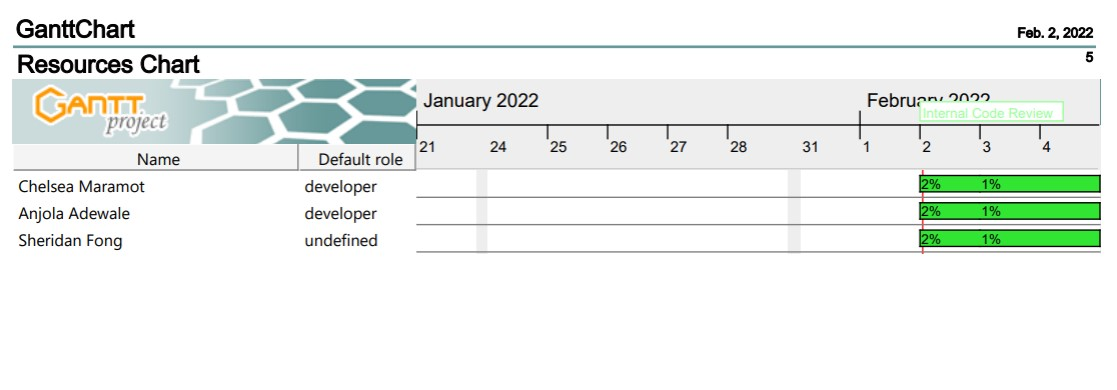
\includegraphics[scale=0.9,angle=90]{resource}
			\caption{Team Rex Resource Distribution}
		\end{figure}		
	
	
	\section{Project Review}
	\color{blue}
	This project provided a tremendous learning opportunity for all members of Team Rex. Prior to
	Our team dynamic and rapport was amazing and each team member performed all tasks correctly and effectively.
	The GIT work flow plan worked out perfectly and allowed us to track our progress. In addition to creating branches for each new features, we also created git Issues to address and track any bugs. It is important to add that learning how to properly use git was a bit of a hassle at first however persevered and succeeded!
	The project management, team work and software development skills that were gained during this project will continue to prove useful in our future endeavors.
	
	As for development technology, it was a good idea to use Python and Pygame as the primary tools.
	Our team had prior experience with Python, thus learning to use Pygame was a very smooth process. 
	Out team also has excellent and effective communication. Team communication was active during the pre-specified lab time and outside lab hours. The use of Microsoft Teams as a companion website contributed to our effective communication as we were able to keep track of documents and easily schedule meetings.
	
	
	Areas of the improvement include completing Documentations in a timely manner.
	Although, all deliverable were submitted on time and were of good quality, 80\% of them were completed on the due date which induced a lot of stress. Completing the documentation 24hrs prior to the deadline would allow for a buffer period where extensive edits, revisions and updates can be made to the document.
	In addition, for a future project, we would modify the Team member roles to be a little more specific. 
	In the current Team Member roles, no team member is assigned any specific role; we stated that all team members are on both the development and test teams. This is accurate however, including a lead Developer and Lead Tester for each component of our design would provide clarity and enhance organization. Lastly, the selected testing framework was unittest. However we found that a lot of the tests we performed were manual as it is difficult to perform automated tests for programs with graphical user interfaces. Thus further research into testing shoudl be performed before deciding on a testing framework.
	In addition the technology section was a little vague and so for future projects a more detailed technology plan should be implemented.

In conclusion, our team worked exceptionally well together. Tasks were completely promptly and correctly, communications was constant and effective. However, better time management as well as explicitly defining team member roles are areas that need improvement for future projects. The development of this project was a great learning experience and the skills developed during its will be utilized in future projects
	
\end{document}
